\chapter{相关概念及技术介绍}

本软件内核采用 Python 语言编写,插件主要采用 Python 和 C++ 语言编写,部分插件对 OpenCV、FFmpeg 等项目产生了依赖,用到了 GoogleNet 等深度学习结构。下面将对这几个部分的内容分别做简要的介绍。

\section{Python 概述}

Python 是一种解释型、面向对象、静态类型的高级编程语言,支持多种编程范式,包括结构化程序设计、过程化程序设计、反射式程序设计、面向对象程序设计和函数式程序设计等 \cite{wiki_py}。它的高级内置数据结构与动态类型和动态绑定相结合,使其非常适合应用于快速应用程序开发以及用作脚本或胶水语言以将现有组件连接在一起 \cite{whats_py}。

Python 以其简洁而清晰的语法著称,这使得代码易于编写和阅读。简明的语法规则和可读性强的代码风格使开发者能够更快速地理解和维护代码,从而提高开发效率 \cite{about_py}。随着时间的推移,Python 不断演变和改进,发展出了丰富的标准库和第三方库,使得它在各个领域都得到了广泛应用,特别是在数据分析、计算机视觉、机器学习等领域,Python 变得极为流行 \cite{pep206}。

\section{C++ 概述}

C++ 是一种编译型、面向对象、静态类型的高级编程语言,支持多重编程范式,包括过程化程序设计、面向对象程序设计、泛型程序设计和函数式程序设计等 \cite{wiki_c}。

起初,这种语言作为 C 语言的增强版出现,被称作 “C with Classes”,即“包含‘类’的 C 语言” \cite{bs_c}。C++ 拥有与 C 语言相同的底层控制能力,它支持直接的硬件访问和低级操作,使得开发者可以编写高性能的代码,并充分利用计算机系统的资源;同时,面向对象的 C++ 程序的速度与用 C 语言写的程序的速度相差在 10\% 以内,而且常常更接近 \cite{t_c}。

\section{OpenCV 概述}

OpenCV,全称为 Open Source Computer Vision Library,即开源计算机视觉库。OpenCV 是一个跨平台的计算机视觉和机器学习编程函数库 \cite{rcv}。OpenCV 是自由软件,通过 Apache 2 许可证开源。

OpenCV 用 C++ 编写,它的主要接口也是 C++。但是,它依然保留了大量的 C 语言接口。同时,它也有 Python、Java、MATLAB、C\#、Ruby 等语言的接口 \cite{wiki_opencv}。OpenCV 倾向于为实时视觉应用程序服务,支持 MMX 和 SSE 指令。目前,OpenCV 开发团队正在积极开发功能齐全的 CUDA 和 OpenCL 接口 \cite{opencv_about}。

OpenCV 拥有 2500 多个优化算法。无论是经典的计算机视觉和机器学习算法,还是最先进的计算机视觉和机器学习算法,都包括在 OpenCV 库中 \cite{opencv_about}。这些算法的功能包括:

\begin{enumerate}
    \item 检测和识别人脸。
    \item 检测和识别物体。
    \item 对视频中的人类动作进行分类。
    \item 跟踪摄像机运动。
    \item 跟踪移动物体。这和跟踪摄像机运动是有区别的。跟踪摄像机运动功能是从视频拍摄角度出发,跟踪移动物体功能是从被拍摄的物体角度出发。
    \item 提取物体的 3D 模型。
    \item 从立体摄像机生成 3D 点云。
    \item 将图像拼接在一起,以生成整个场景的高分辨率图像。
    \item 从使用闪光灯拍摄的图像中去除红眼。
    \item 识别背景并进行标记,以将其与增强现实(Augmented Reality, AR)叠加。
\end{enumerate}

该库被广泛应用于商业。除了谷歌、雅虎、微软、英特尔、IBM、索尼、本田、丰田、腾讯、字节跳动等知名公司外,还有如 Applied Minds、VideoSurf 和 Zeitera 等许多初创公司使用 OpenCV 库 \cite{opencv_about}。

\section{FFmpeg 概述}

FFmpeg 是一个跨平台的开源多媒体框架,能够编码(encoding)、解码(decoding)、转码(transcode)、复用(mux)、解复用(demux)、流式传输(stream)、过滤(filter)和播放(play)人类和机器创造的几乎所有多媒体内容 \cite{ffmpeg_about}。FFmpeg 包括它的工具和库。

FFmpeg 工具包括 \cite{ffmpeg_doc}:

\begin{enumerate}
    \item 命令行工具 ffmpeg。ffmpeg 是一种通用的多媒体转换器,用于在格式之间转换多媒体文件。它可以读取各种输入,包括实时抓取记录设备,然后过滤并将它们转码为多种输出格式。
    \item 命令行工具 ffplay。ffplay 是一种通用的多媒体播放器,基于 SDL 和 FFmpeg 库。
    \item 命令行工具 ffprobe。ffprobe 是一种通用的多媒体分析器。它多媒体流中收集信息,并以人类和机器可读的方式打印出来。它可用于检查多媒体流使用的容器格式以及其中包含的每个媒体流的格式和类型。
\end{enumerate}

\begin{figure}[h]
    \centering
    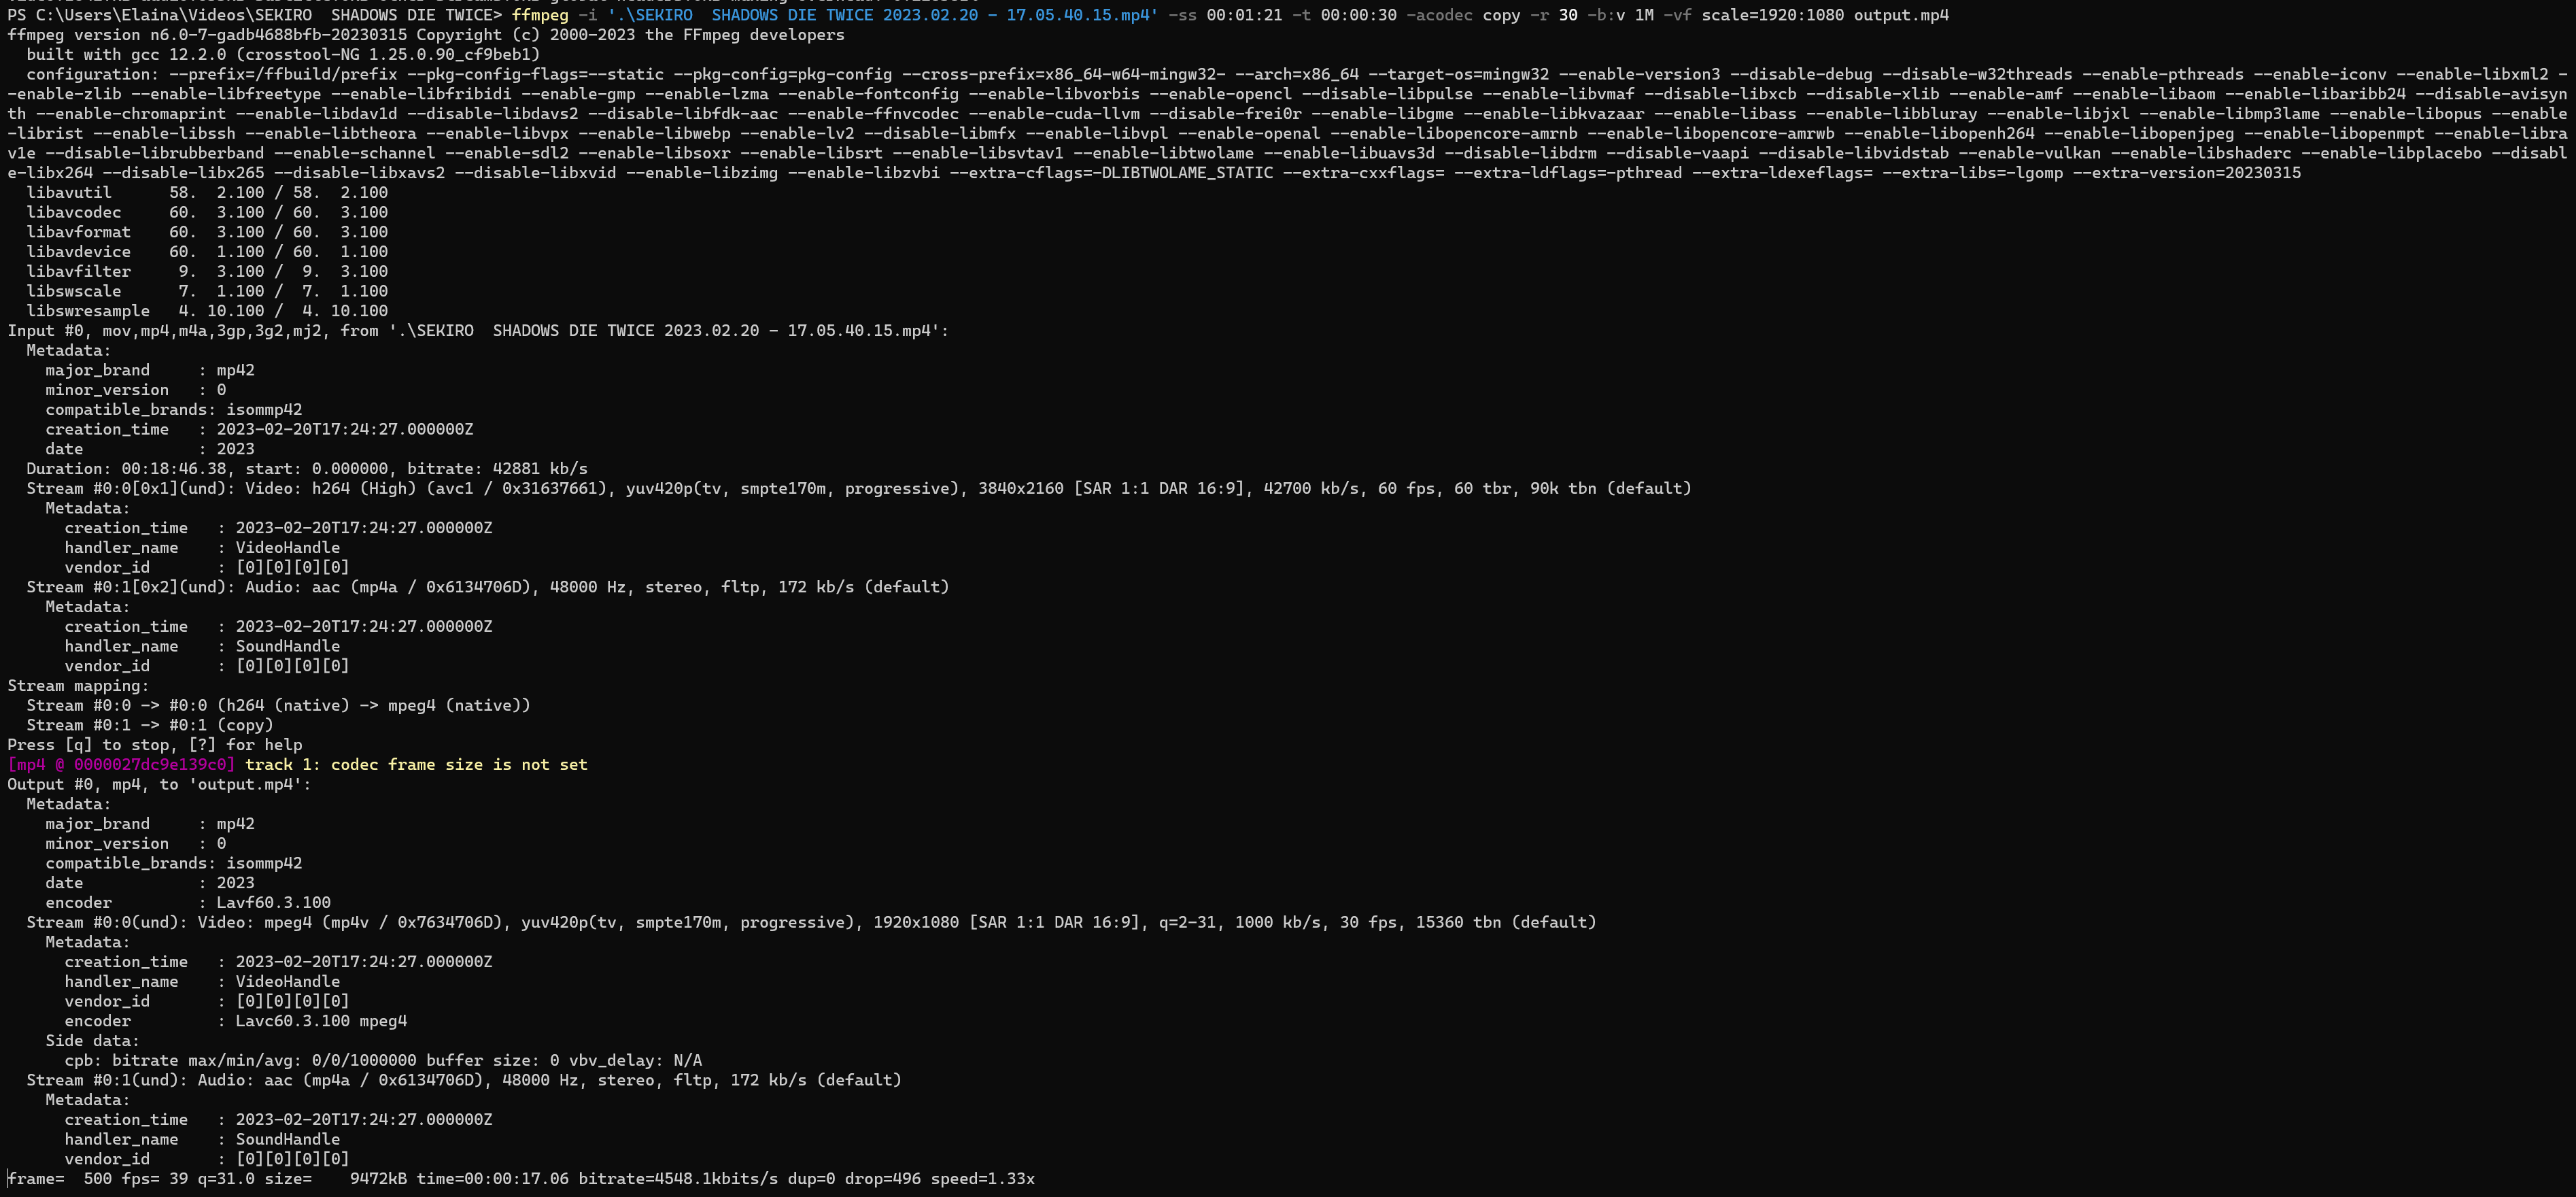
\includegraphics[width=\textwidth]{figures/ffmpeg.png}
    \caption{使用命令行工具 ffmpeg 处理视频}
    \label{fig:ffmpeg}
\end{figure}

FFmpeg 库包括 \cite{ffmpeg_doc}:

\begin{enumerate}
    \item 库 libavutil。libavutil 是一个用于辅助便携式多媒体编程的实用程序库。它包含可安全移植的字符串函数、随机数生成器、一些数据结构、附加的数学函数、密码学和多媒体相关功能。它可以简化编程,便于开发人员调用并开发。为了降低相互依赖性,它不是 libavcodec 和 libavformat 所需代码的库。
    \item 库 libavcodec。libavcodec 是一个包含音频、视频的解码器和编码器的库。它提供了一个通用的编码和解码框架(framework),并包含用于音频流、视频流和字幕流的多个解码器和编码器,以及多个比特流(bitstream)过滤器。它的共享架构(shared architectur)提供从比特流 I/O 到数字信号处理器(digital signal processor, DSP,是一种专用于数字信号处理的微处理器)优化的服务,使其适用于实现稳健和快速的编码器和解码器 \cite{libavcodec}。
    \item 库 libavformat。libavformat 是一个包含多媒体容器格式的复用器和解复用器的库。它为音频流、视频流和字幕流的多路复用(multiplexing)和多路分解(demultiplexing)提供了一个通用框架。它提供了多种输入和输出协议,来访问媒体资源。它提供了一些通用的全局选项,可以在所有协议上设置。它包含用于多媒体容器格式的多个复用器和解复用器。
    \item 库 libavdevice。libavdevice 是一个包含输入和输出设备的库。它提供了一个通用框架,用于从许多常见的多媒体输入设备中获取(grabbing)获取输出,以及从许多常见的多媒体输出设备中渲染(rendering)设备。它提供了与库 libavformat 相同的接口,即输入设备被视为多路分解器,输出设备被视为多路复用器。它支持包括 \tt{Video4Linux2}、\tt{VfW}、\tt{DShow} 和 \tt{ALSA} 在内的多种输入和输出设备。
    \item 库 libavfilter。libavfilter 是一个包含媒体过滤器的库。它提供了一个通用的音频、视频过滤框架,其中包含多个过滤器、源(source)和接收器。一个过滤器可以有多个输入和输出。当没有输入或输出时,可以使用源头过滤器 \tt{source filter} 或接收过滤器 \tt{sink filter}。
    \item 库 libswscale。libswscale 是一个用于图像缩放和像素(pixel)格式转换的库。
    \begin{enumerate}
        \item 它可以改变视频的分辨率,有多种重新缩放选项和算法可用。在缩放的过程中,可以为不同的分量选择不同的算法。在实现的过程中,这些算法被高度优化。% 它支持双线性缩放算法(bilinear scaling algorithm)、快速双线性缩放算法(fast bilinear scaling algorithm)(此处的“快速”指通过降低缩放标准来降低时间复杂度,而不是同一算法的更优实现)、双三次缩放算法(bicubic scaling algorithm)、经验缩放算法(experimental scaling algorithm)、最近邻重新缩放算法(nearest neighbor rescaling algorithm)、平均面积重新缩放算法(averaging area rescaling algorithm)、高斯重新缩放算法(Gaussian rescaling algorithm)、正弦波重新缩放算法(sinc rescaling algorithm.)、兰佐斯重新缩放算法(Lanczos rescaling algorithm)、自然双三次样条重新缩放算法(natural bicubic spline rescaling algorithm)。
        \item 它可以将转换图像的格式和色彩空间(color space,色彩的组织方式),例如从 \tt{BGR24} (bule green red 24 bits per pixel, bule green red 24 BPP,是一种 sRGB 格式,具有 3 个色彩通道(channel),每个色彩通道每像素具有 8 位信息)转换到 \tt{GRAY}(灰度),如果源色彩空间和目标色彩空间不同,这通常是一个有损(lossy)过程 \cite{bgr24}。
        \item 它还可以处理布局转换,即从打包布局(packed layout,属于不同平面的所有像素存储在同一缓冲区(buffer)中)转换为平面布局(planar layout,属于同一平面的像素存储在专用缓冲区中,属于不同平面的像素存储在不同缓冲区中)。
    \end{enumerate}
    \item 库 libswresample。libswresample 是一个用于音频重采样(resampling)、音频通道布局重新矩阵化(rematrixing)、样本格式转换和打包布局的库。
    \begin{enumerate}
        \item 它可以转换音频采样率,有多种重采样算法和选项可供选择。当从高采样率转换到低采样率时,这是一个有损过程。
        \item 它可以转换像素类型。例如,从 8 位无符号整数(uint8)类型转换到 16 位有符号整数(int16)类型,或转换到 32 位浮点(float32)类型。
        \item 它可以改变通道布局,例如从立体声到单声道。当输入通道不能映射到输出流时,这个过程是有损的,因为它涉及不同的增益因子(gain factors,用于限制扬声器的信号以获得更好的放大效果,当设置错误时将会导致音频失真)和音频混合 \cite{gain}。
    \end{enumerate}
    它可以通过专用选项使用各种其他音频转换功能,例如音频拉伸(stretching)和填充(padding) 。
\end{enumerate}

\section{GoogLeNet 概述}

GoogLeNet 是一种深度学习结构,有 22 层深度。

在 GoogLeNet 提出之前,流行的 AlexNet、VGGNet(VGG-16) 等深度学习结构都是通过增大网络的深度(层数)来获得更好的训练效果,但层数的增加会带来很多负作用 \cite{alexnet} \cite{vgg}。

GoogLeNet 则是从另一种角度来提升训练结果。GoogLeNet 可以更高效地利用计算资源,在相同的计算量下,它可以提取到更多的特征,从而提升训练结果。在 GoogLeNet 的结构中,整个 Inception 结构由多个 Inception 模块串联起来。Inception 结构使用 $1\times1$ 的卷积来进行升降维,这是因为在相同尺寸的感受野中叠加更多的卷积,能提取到更丰富的特征 \cite{nin}。同时,Inception 结构在特征维度上进行分解,将相关性强的特征汇聚到一起,在多个尺寸上同时进行卷积再聚合 \cite{ggnet1}。

\begin{figure}[h]
    \centering
    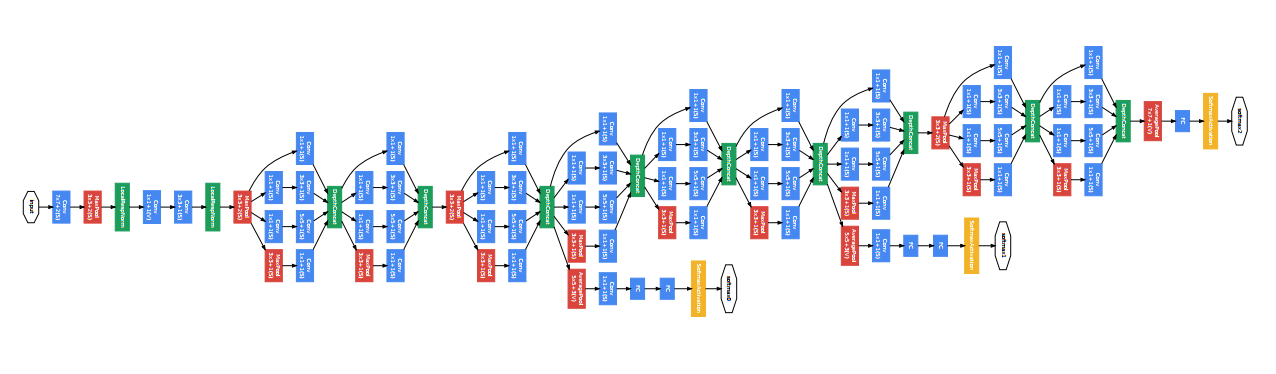
\includegraphics[width=\textwidth]{figures/arch.png}
    \caption{GoogLeNet 架构}
    \label{fig:arch}
\end{figure}

GoogLeNet 支持迁移学习,可以自行重新训练 GoogLeNet 网络来执行一个新任务 \cite{ggnet1}。

目前,GoogLeNet 正变得流行,Caffe、TensorFlow 和 Torch 等深度学习框架以及科学计算语言 MATLAB 均直接提供了 GoogLeNet 的算法支持,部分还提供了预训练模型支持。
